\chapter{Detekcia osôb}
\label{kap:detection}
Detekciu definujeme ako identifikáciu regiónu na vstupnej snímke, v ktorom sa nachádza hľadaný objekt.
Predtým, ako osobu na zázname môžeme rozpoznávať a sledovať, je potrebné ju detegovať.
Jedná sa o dôležitý problém, ktorý je možné riešiť viacerými spôsobmi.

\section{Haarove príznaky}
Isté časti objektov, ktoré chceme detegovať, sú tmavšie ako iné časti.
Túto skutočnosť zachytávajú haarove príznaky.

Haarove príznaky si vieme predstaviť ako obĺžniky, ktoré obsahujú dva typy regiónov.
V oboch regiónoch sa sčítajú hodnoty pixelov a výsledný príznak je rozdiel týchto súčtov.
Pri detekcii pomocou haarových príznakov sa zoberú všetky možné veľkosti a pozície takýchto obdĺžnikov.

Pre urýchlenie výpočtu súm sa využije metóda integrálneho obrazu.
V integrálnom obraze $I$ predstavuje hodnota pixelu súčet všetkých pixelov nachádzajúcich sa vľavo a nad od tohto pixelu v pôdovnom obraze $O$.
$$I(x, y) = \sum_{i=1}^{x} \sum_{j=1}^{y} O(x, y)$$
Ak chceme vypočítať súčet pixelov obĺžnikového regiónu. stačia nám tri operácie sčítania a odčítania.
Od spodného pravého pixelu odpočítame hodnoty ľavého dolného a pravého horného pixelu od ľavého dolného pixelu a následne ešte pričítame hodnotu ľavého horného pixelu.

\begin{figure}[H]
\centerline{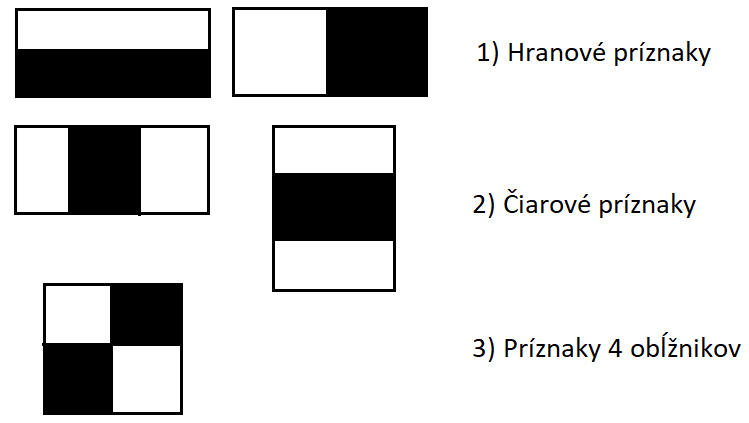
\includegraphics[width=0.9\textwidth]{images/haar}}
\caption[Haarove príznaky]{Ukážka troch typov haarovych príznakov, ktoré sa používajú na detekciu tváre algoritmom Viola-Jones \cite{violajones}. Súčet hodnôt pixelov v bielych regiónov je odčítaný od súčtu hodnôt pixelov v čiernych regiónov.}
\label{obr:haar}
\end{figure}

Na vstupnom obraze veľkú časť zaberajú regióny, v ktorých sa hľadaný objekt nenachádza a preto by bolo testovanie všetkých príznakov zbytočné.
Je preto zavedený kaskádový systém, kde sa v prvej fáze otestuje len niekoľko príznakov a pokiaľ sa určí, že na tomto regióne sa hľadaný objekt nenachádza, prejdeme na ďalší región a hľadáme ďalej.
V opačnom prípade kaskádovo pokračujeme testovaním presnejších príznakov \cite{violajones}. 

\section{Histogram orientovaných gradientov}
Hlavnou myšlienkov je, že zachytenie distribúcie orientácie a intenzity gradientov v snímke dokáže popísať tvar hľadaného objektu.

Vstupná snímka je rozdelená na regióny rovnakej veľkosti.
Následne sa v každom regióne vypočítajú orientácie gradientov a tie sa zaznamenajú v histograme.
Intenzita určuje váhu orientácie v gradiente, čiže gradienty s malou interzitou vytvorené napríklad šumom nie sú pri výpočte podstatné.

Jednotlivé regióny sú navyše spájané do skupín, ktoré sa môže prelínať, čo znižuje vplyv zmien osvetlenia na snímke.
Prelínanie redukuje rozdiely medzi jednotlivými skupinami a v praxi sa ukazuje, že takéto riešenie dosahuje lepšie výsledky \cite{hogov}.
Spojením výsledných histogramov jednotlivých skupín vznikne výstupný vektor príznakov - histogram orientovaných gradientov \cite{hog1} \cite{hog2}.

\begin{figure}[H]
\centerline{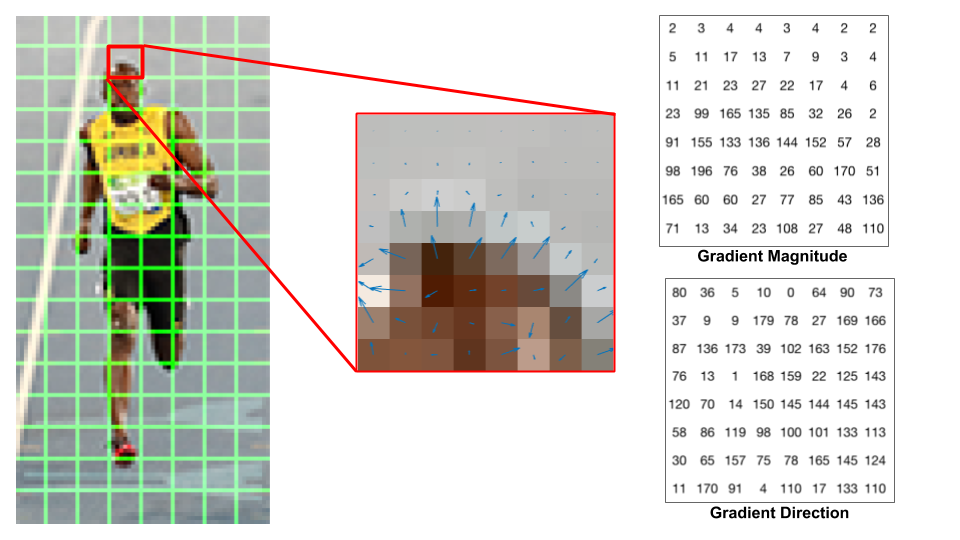
\includegraphics[width=0.9\textwidth]{images/hog_example}}
\caption[Ukažka výpočtu histogramu orientovaných gradientov]{Ukažka výpočtu histogramu orientovaných gradientov. Pre každý región je sú vypočítaný gradienty reprezentované orientáciou a intenzitou \cite{hogov}.}
\label{obr:hog_example}
\end{figure}

\section{Konvolučné neurónové siete}
Neurónové siete vyžadujú na ich natrénovanie veľký počet označených dát.

Ak chceme natrénovať neurónovú sieť, ktorá hľadá na snímkach postavy ľudí, potrebujeme snímky s označenými obdĺžnikami ohraničujúcimi časti snímok, na ktorých sa postavy ľudí nachádzajú.
Tomuto postupu hovoríme učenie s učitelom.
Trénovanie prebieha pokusom a omylom. 
V každej iterácii sieť vyskúša spraviť predikciu na trénovavích príkladoch a vypočíta rozdiel medzi predikciou a očakávaným výstupom.
Cieľom je v najsledujúcej iterácii túto chybu znížiť.
Na meranie úspešnosti predikcii sa používa stratová funkcia \cite{cnn1}.

Neurónová sieť sa skladá zo vstupnej a výstupnej vrstvy, medzi ktorými je niekoľko skrytých vrstiev.
V konvolučných neurónových sieťach sa vyskytujú vrstvy, ktorých úlohou je detegovať hrany, tvary, farby a podobne.
Tieto vrstvy nazývame konvolučné vrstvy.

V konvolučných vrstvách je dôležitý pojem filter.
Filter je matica váh, ktorou sa prenásobujú podregióny vstupu do vrstvy rovné veľkosti filtra.
Podregióny vznikajú metódou pohybujúceho sa okna, začneme v ľavom hornom roku a postupne sa posúvame o jeden prvok.
Tento proces sa nazýva konvolúcia \cite{cnn2}. 
Pre každú konvolučnú vrstvu máme definovaný počet a veľkosť filtrov.

S využitím väčšieho množstva konvolučných vrstiev zostrojíme sieť, ktorá dokáže rozpoznávať aj komplikovanejšie vzory.
Medzi konvolučnými vrstvami zvyčajne máme ďalšie vrstvy ako sú ReLU vrstvy a vrstvy redukujúce dimenziu.

Na konci siete sa nachádza plne-prepojená vrstva, ktorá spája výstupy filtrov z predchádzajúcej konvolučnej vrstvy, prípadne výstupov ďalších vrstiev, ktoré sa môžu nachádzať po tejto konvolučnej vrstve.

\begin{figure}[H]
\centerline{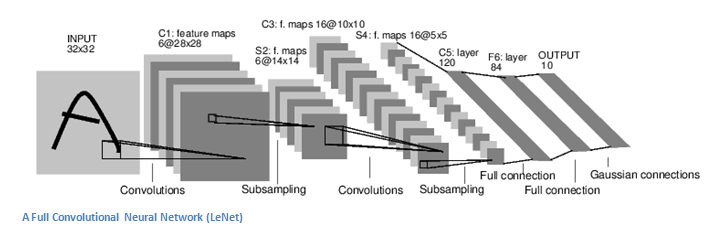
\includegraphics[width=0.9\textwidth]{images/conv}}
\caption[Konvolučná neurónová sieť]{Ukážka architektúry jednoduchej konvolučnej neurónovej siete \cite{cnn2}.}
\label{obr:conv}
\end{figure}

\section{Porovanie}
Tri popísané typy detekcie sme otestovali pri detekcii postáv na obrázku s rozmerom 3780x2127 pixelov.
Pri haarovych príznakoch a histograme orientovaných gradientov sme využili knižnicu OpenCV a jej zabudované funkcie.
Na detekciu neurónovou sieťou sme využili predtrénovanú neurónovú siet MobileNet-SSD.

Z nižšie uvedenej tabuľky a obrázkov jednoznačne vidieť lepšie výsledky pri detekcii pomocou neurónovej siete.



\begin{table}[H]
\begin{center}
\caption[Namerané časy detekcie]{Namerané časy potrebné na detekciu.}
\begin{tabular}{ |l|r| } 
  \hline
 {Metóda} & {Čas potrebný na detekciu} \\ [0.5ex] 
 \hline
 Haarove príznaky & 168ms \\ 
 Histogram orientovaných gradientov & 8\,188ms \\ 
 Neurónová sieť & 4\,901ms \\ 
 \hline
\end{tabular}
\end{center}
\end{table}


\begin{figure}[H]
\centerline{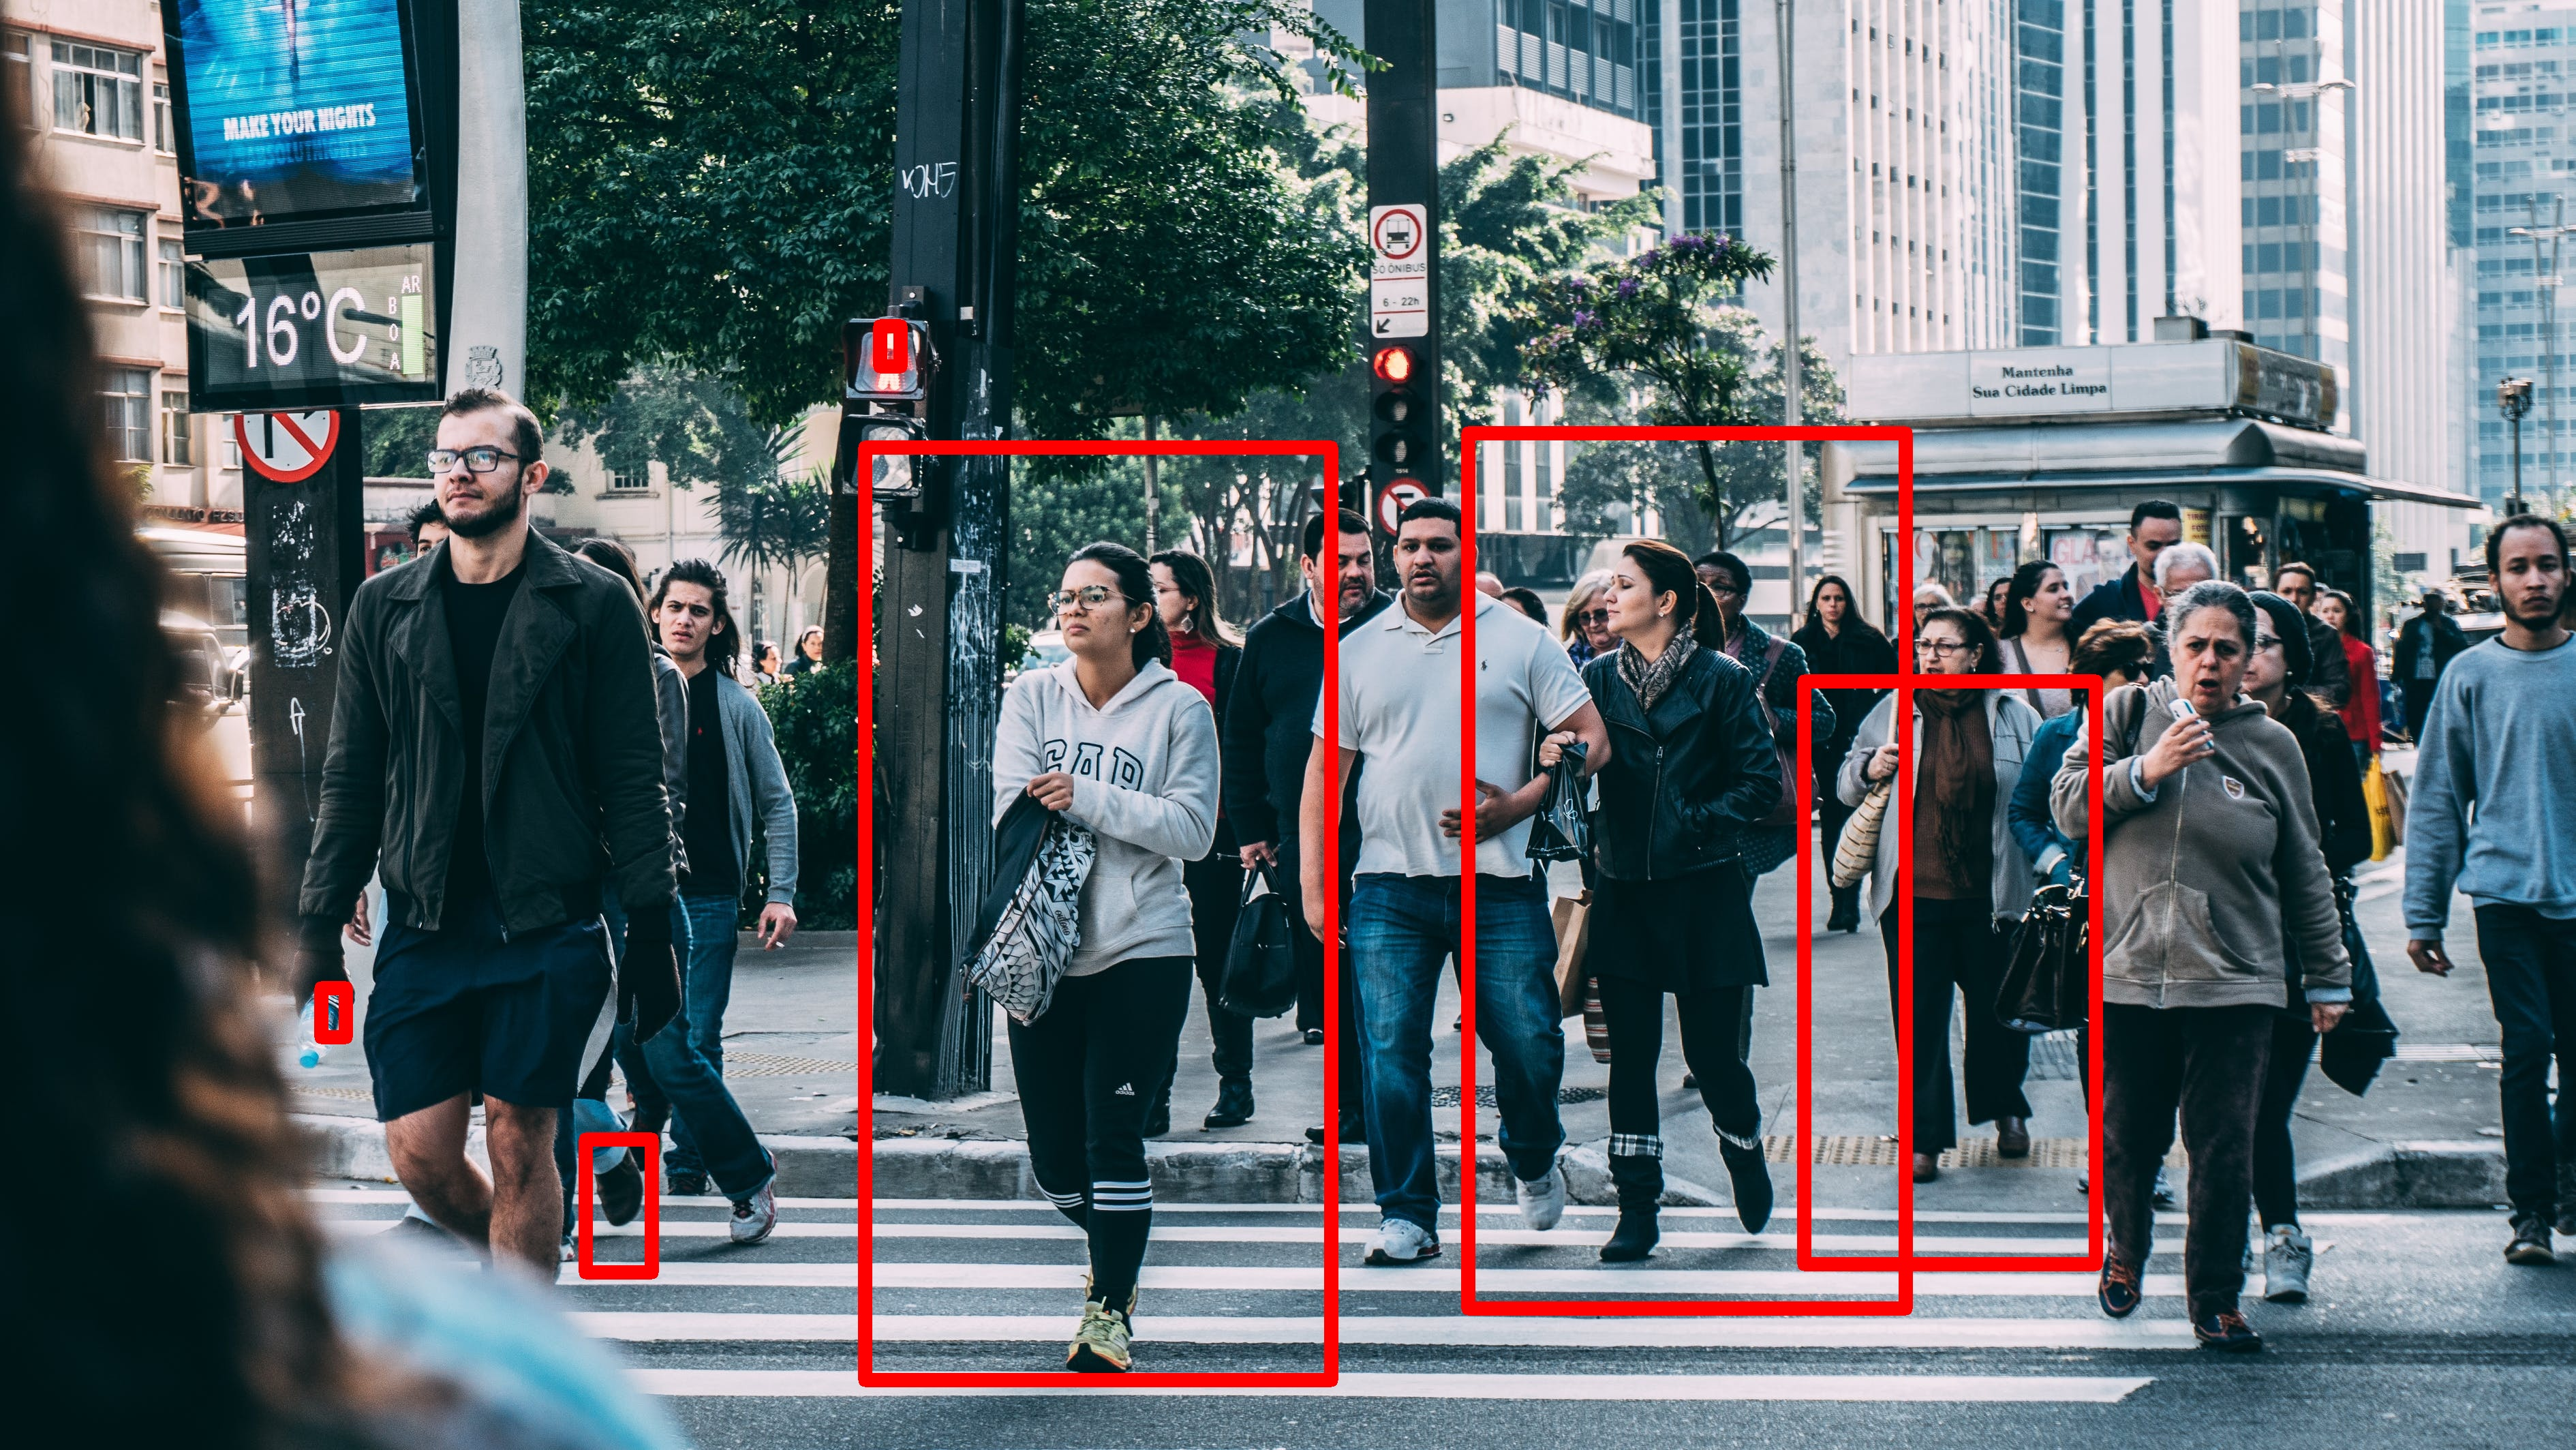
\includegraphics[width=1\textwidth]{images/detect_haar}}
\caption[Detekcia pomocou haarovych príznakov]{Na obrázku vidieť osoby detegované pomocou haarovych príznakov.}
\label{obr:detect_haar}
\end{figure}

\begin{figure}[H]
\centerline{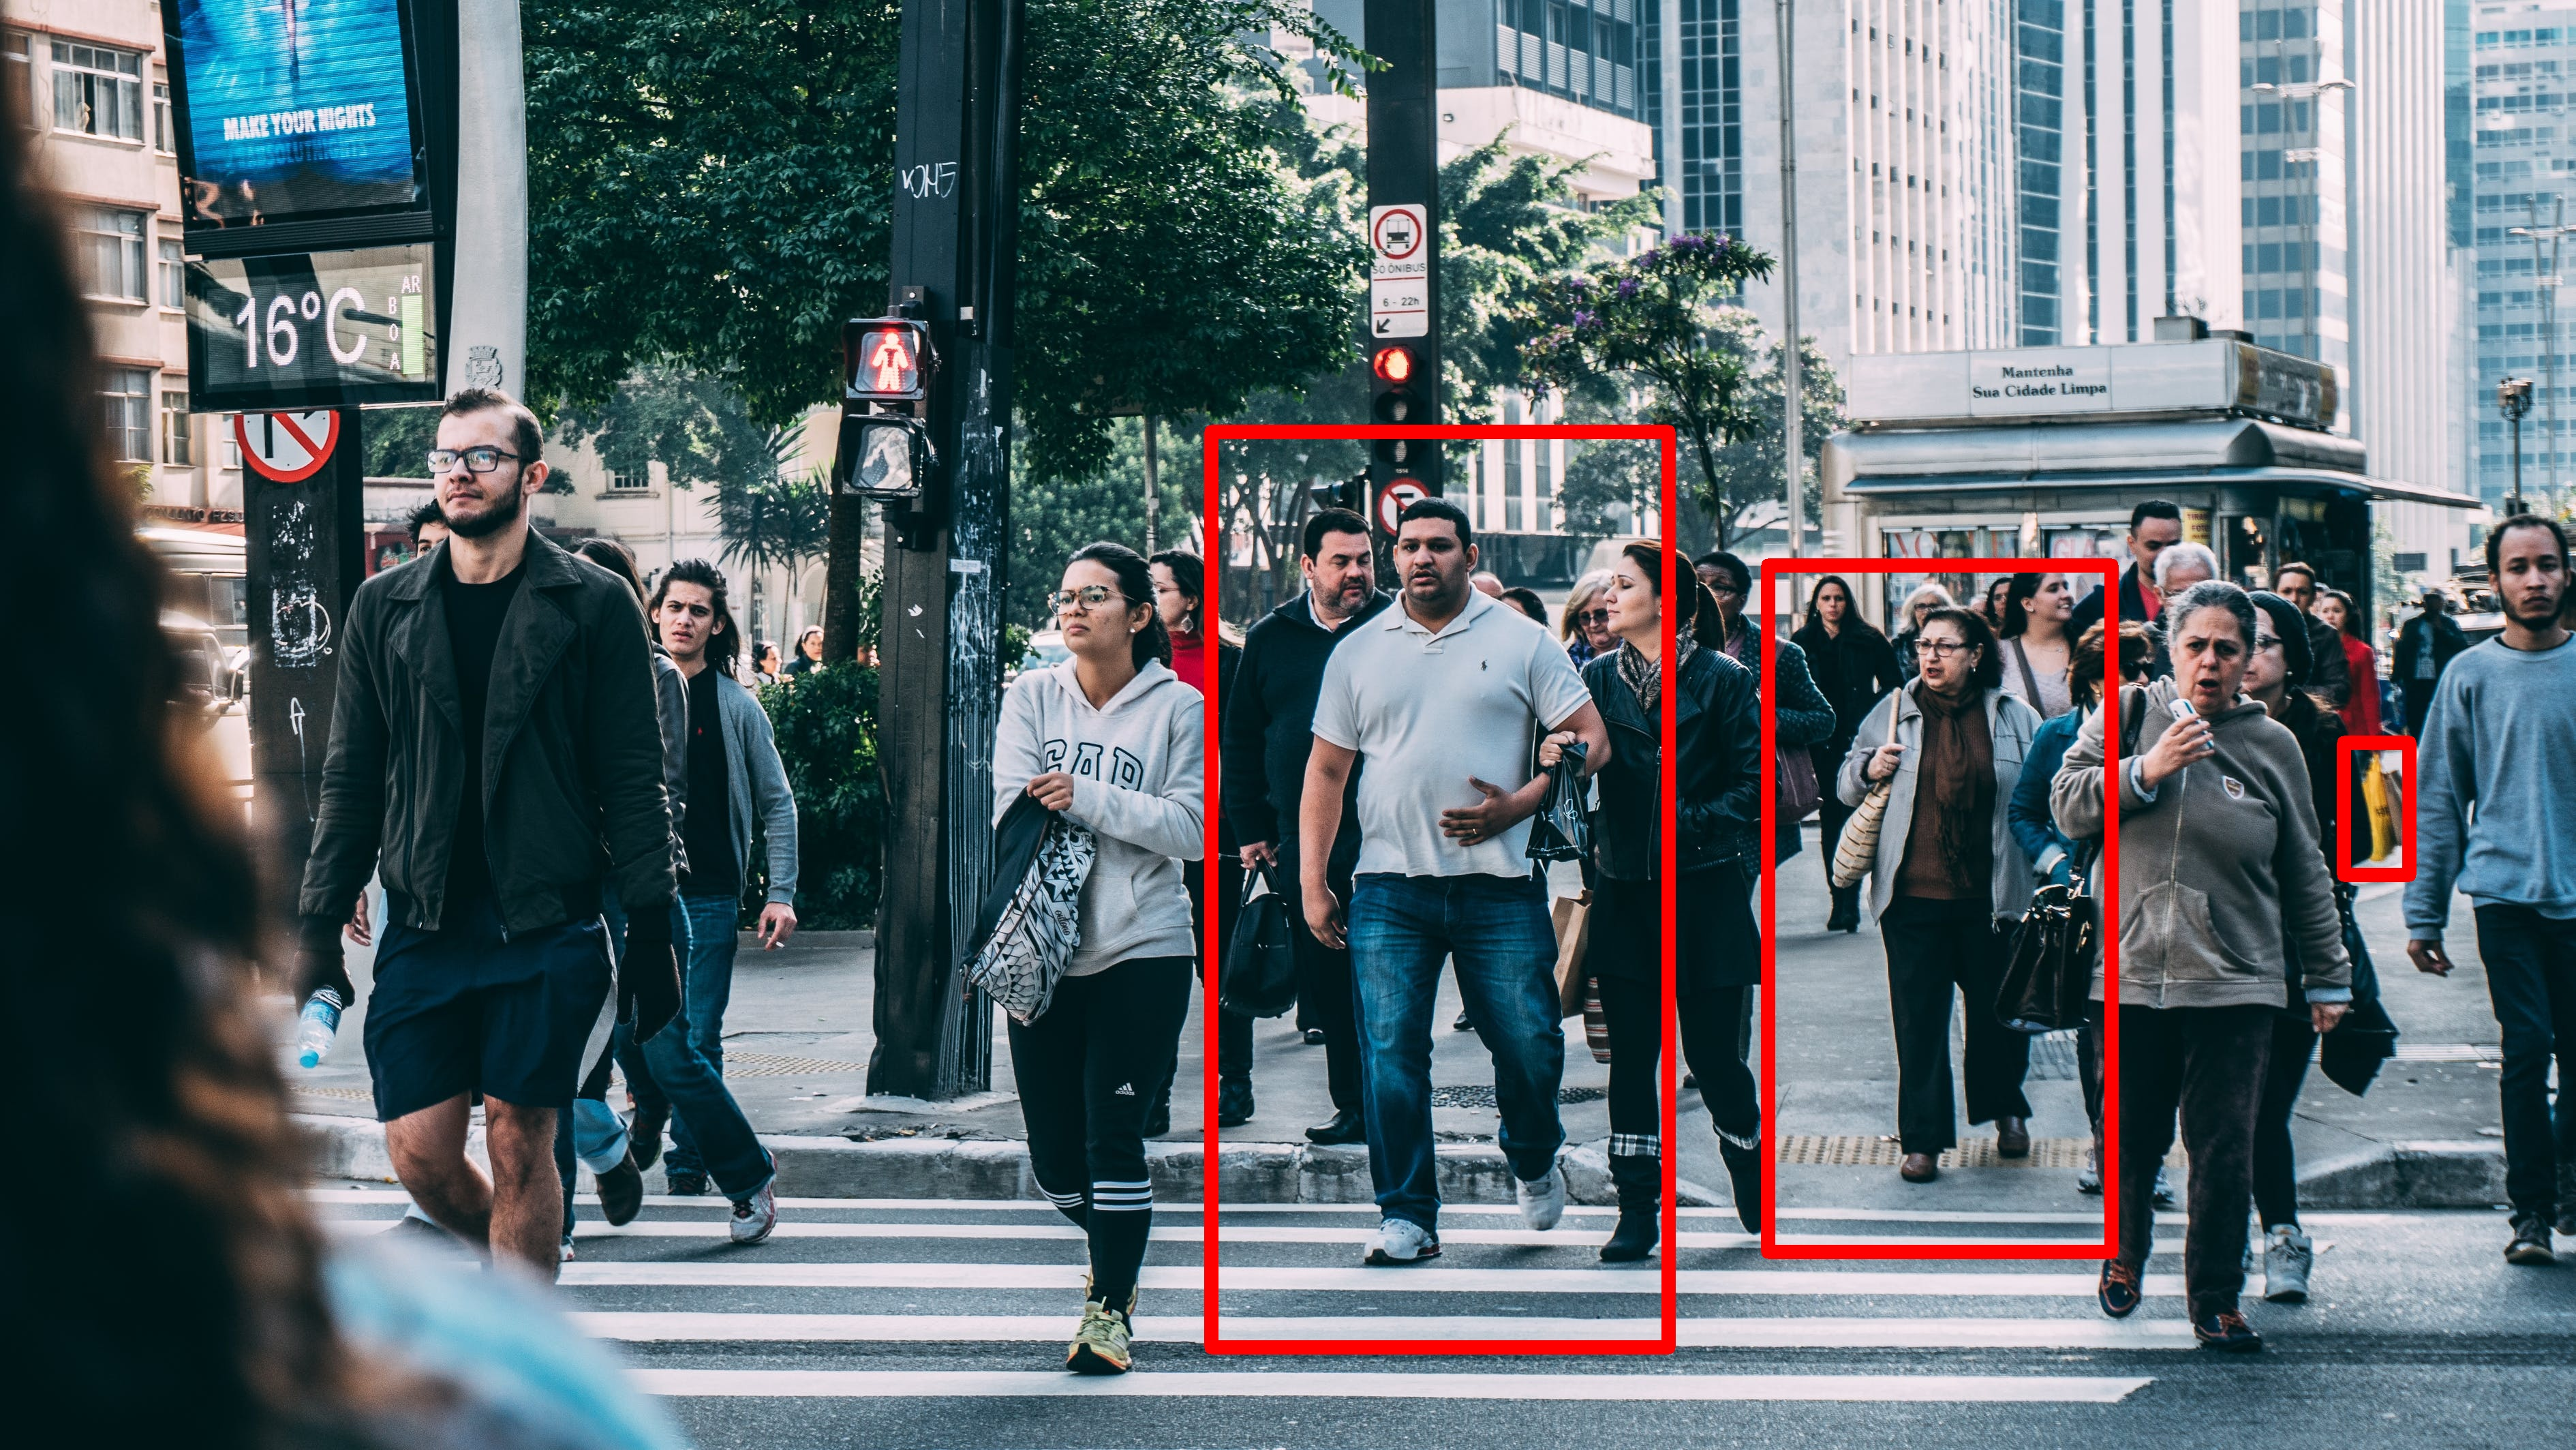
\includegraphics[width=1\textwidth]{images/detect_hog}}
\caption[Detekcia pomocou histogramu orientovaných gradientov]{Na obrázku vidieť osoby detegované pomocou histogramu orientovaných gradientov.}
\label{obr:detect_hog}
\end{figure}

\begin{figure}[H]
\centerline{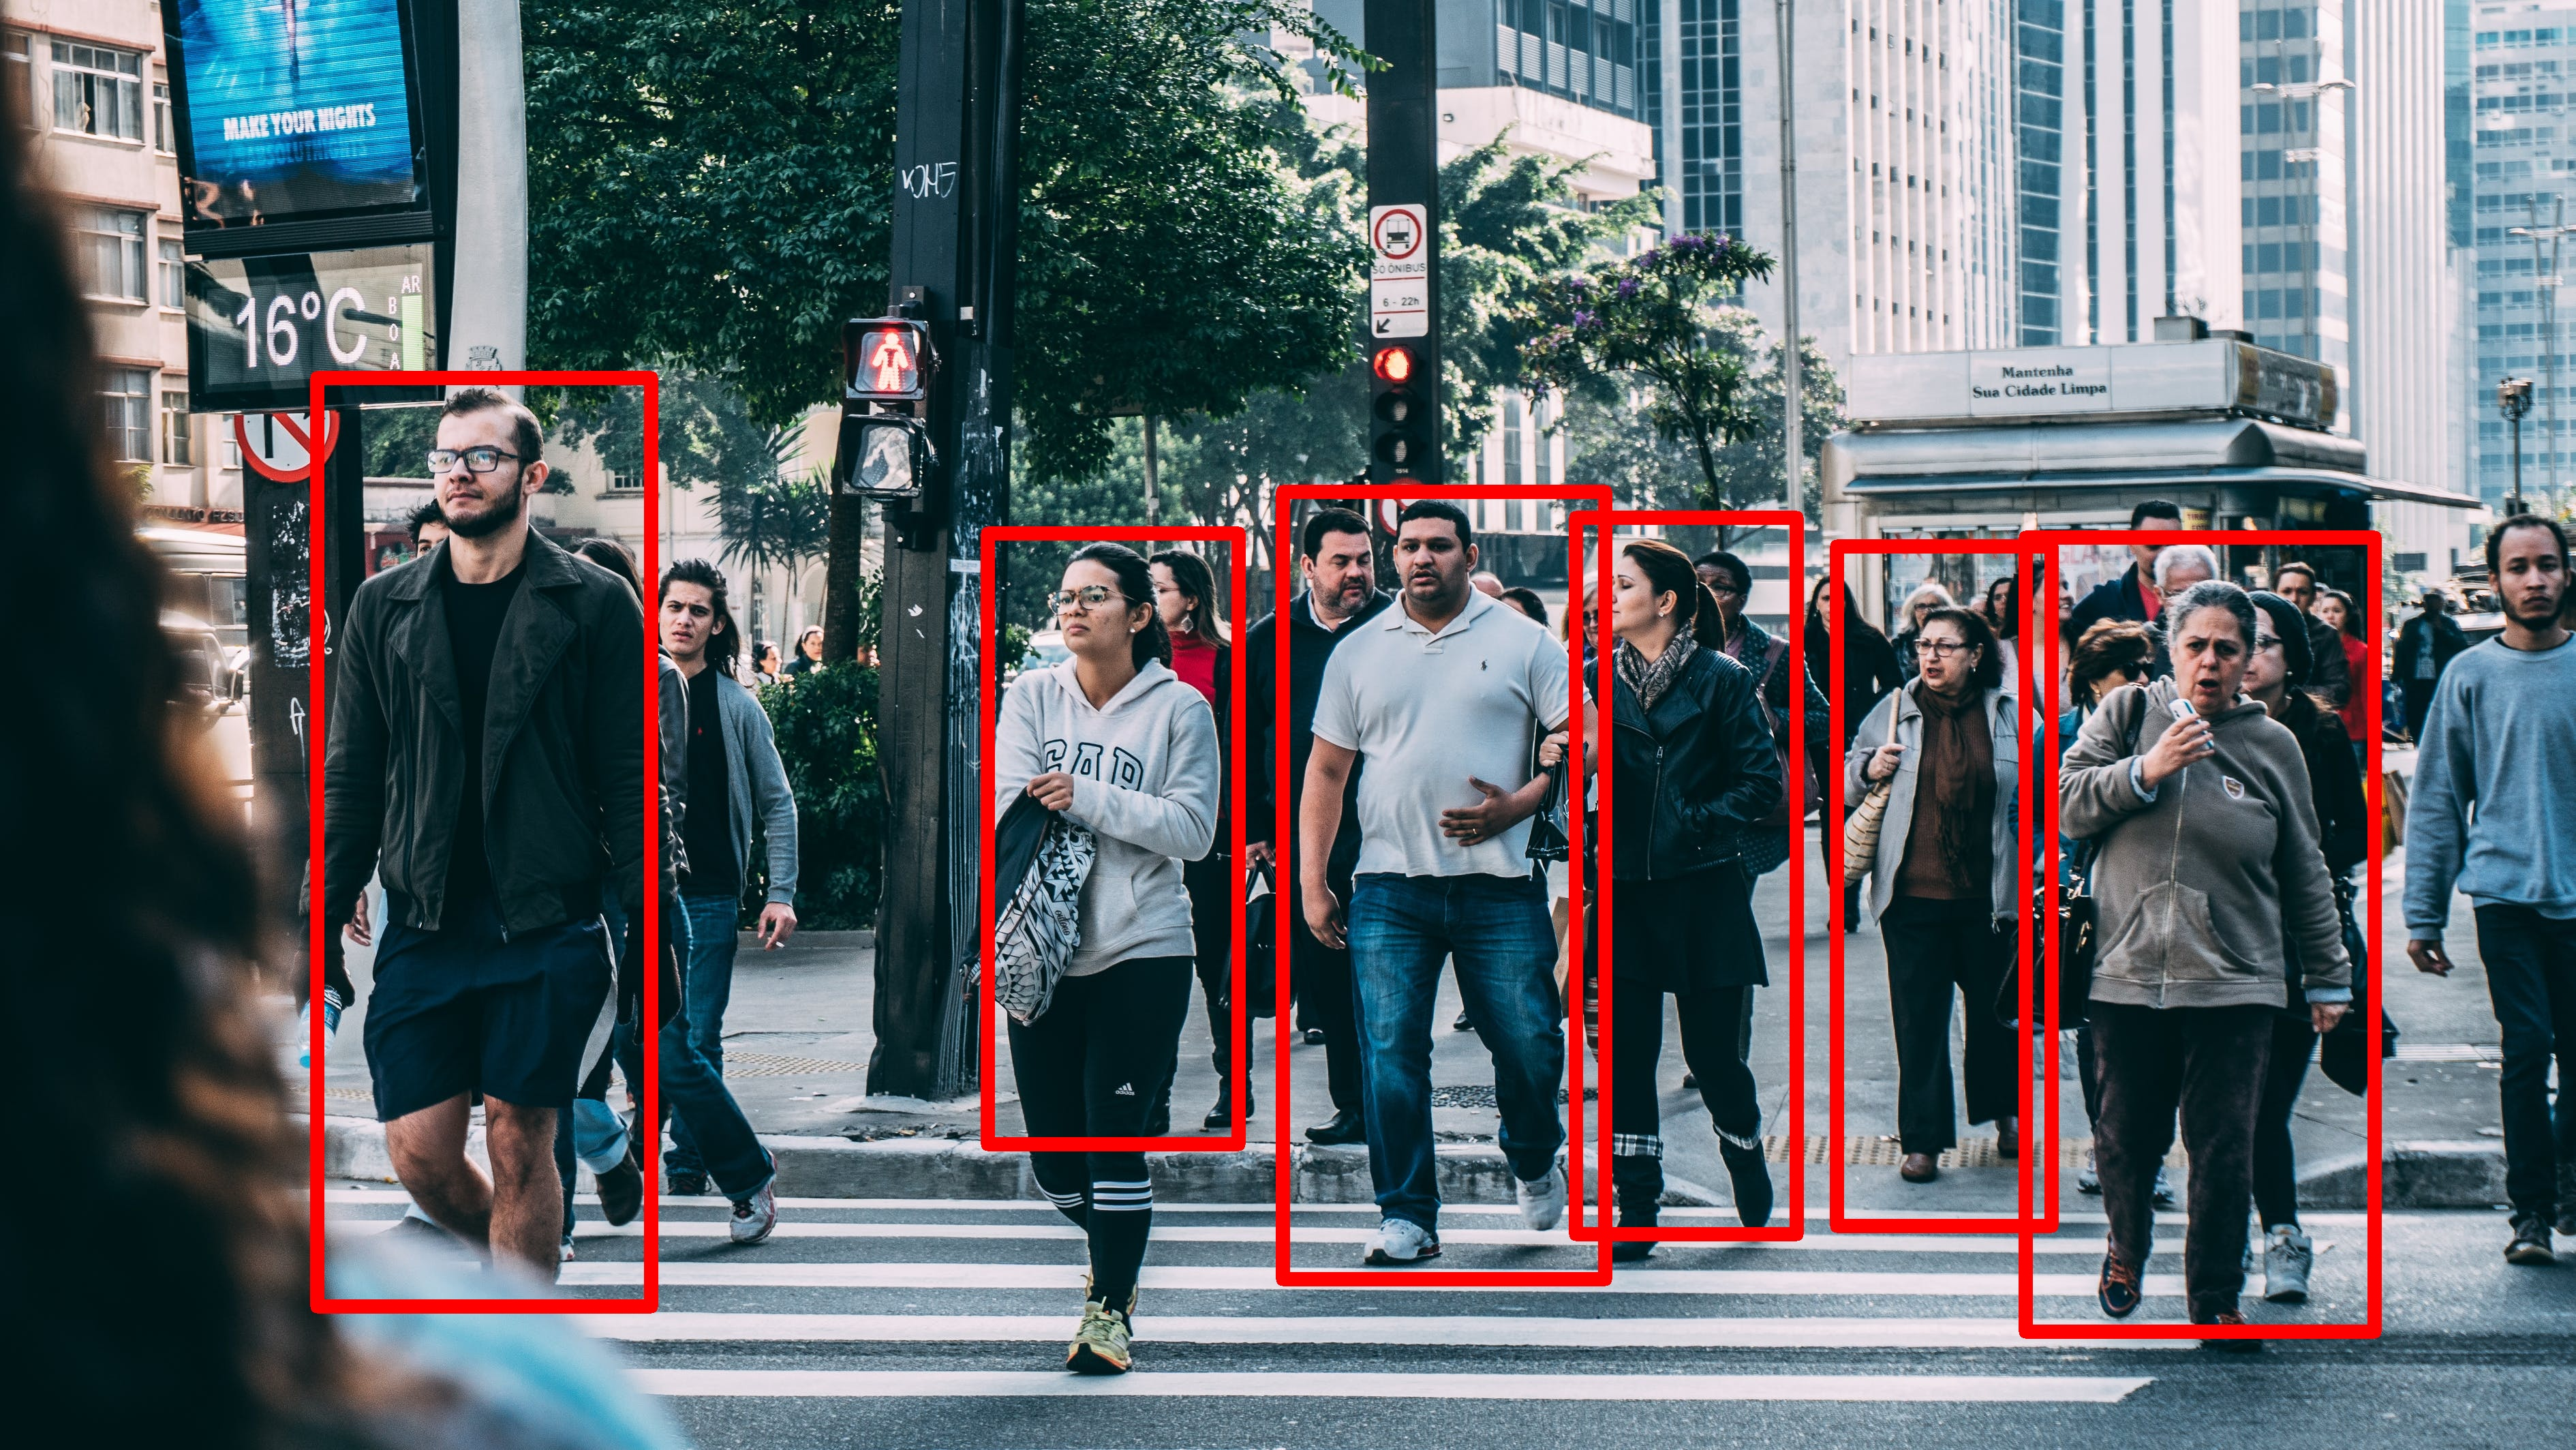
\includegraphics[width=1\textwidth]{images/detect_cnn}}
\caption[Detekcia neurónovou sieťou]{Na obrázku vidieť osoby detegované pomocou neurónovej siete.}
\label{obr:detect_cnn}
\end{figure}